\documentclass[12pt]{article}
\usepackage{class/sbc-template}
\usepackage{graphicx,url}
\usepackage[utf8]{inputenc}
\usepackage[brazil]{babel}
\usepackage{color}
\usepackage{listings}

%%%%%%%%%%%%%%%%%%%%%%%%%%%%%%%%%%%%%%%%%%%%%%%%%%%%
% C O N F I G U R A Ç Õ E S  D O S   C Ó D I G O S %
%%%%%%%%%%%%%%%%%%%%%%%%%%%%%%%%%%%%%%%%%%%%%%%%%%%%

\lstset{
	numbers=left,
	stepnumber=1,
	firstnumber=1,
	numberstyle=\scriptsize,
	extendedchars=true,
	breaklines=true,
	frame=single,
	showstringspaces=false,
  aboveskip=1.5em,
	xleftmargin=2.5em,
	framexleftmargin=2em,
	basicstyle=\scriptsize,
}

\renewcommand{\lstlistingname}{Código}
\renewcommand{\lstlistlistingname}{Lista de Códigos}

\sloppy

\title{Aprendizagem de Máquina (2020/Período Especial) - Impactos da Base de Aprendizagem}

\author{Diogo C. T. Batista\inst{1}}

\address{Universidade Federal do Paraná (UFPR)\\
	Curitiba -- Paraná -- Brasil
	\email{diogo@diogocezar.com}
	}

\begin{document}

\maketitle

\section{Impactos da Base de Aprendizagem}

Esta atividade laboratorial tem como objetivo a investigação exploratória dos impáctos da base de aprendizagem na performance de diferentes classificadores. Os classificadores a serem analisados neste laboratório são:

\begin{itemize}
  \item KNN;
  \item Naïve Bayes;
  \item Linear Discriminant Analysis;
  \item Logistic Regression;
  \item Perceptron.
\end{itemize}

Os dados estão dispostos em arquivo no formato \textit{svmlight}. Este formato dispõe as informações de categorias e suas respectivas características. O código \ref{code:svmlight} mostra um pequeno trecho desta representação.

\begin{lstlisting}[caption={Exemplo do Formato de Entrada},captionpos=b,frame=single,label={code:svmlight}]
0 1:0.000000 2:0.000000 3:0.001412 4:0.000000 5:0.014124 6:0.000000 ...
\end{lstlisting}

Neste exemplo, pode-se notar que o $0$ inicial mostra a qual categoria este dado pertence, na sequência, demonstra-se para cada característica o seu valor. A característica $1$ possui o valor $0.000000$.

Os dados utilizados neste experimento estão dividos em 2 partições. A primeira partição possui $20.000$ registros, que foi definida para uma base de treinamento. Já a segunda, possui $58.646$, utilizados para o teste dos classificadores.

\newpage

\subsection{Estratégia para execução do experimento}

Para automatização dos experimentos, foi criado um sistema \textit{orquestrador} no qual é possível definir as instruções para a execução de todo o fluxo para os 5 diferentes classificadores. O Código \ref{code:orquestrador} mostra os valores definidos em um arquivo no formato \textit{JSON}.

\begin{lstlisting}[caption={JSON do Orquestrador},captionpos=b,frame=single,label={code:orquestrador}]
[
  {
    "classifier": "knn",
    "chunk_start": 1000,
    "chunk_stop": 20000,
    "chunk_step": 1000
  },
  {
    "classifier": "naive\_bayes",
    "chunk_start": 1000,
    "chunk_stop": 20000,
    "chunk_step": 1000
  },
  ...
]
\end{lstlisting}

Neste JSON, \textit{classifier} é o nome do classificador que deve ser utilizado. Estes, podem variar entre: \textit{knn}, \textit{naive\_bayes}, \textit{lda}, \textit{logistic\_regression}, e \textit{perceptron}. Os outros atributos servem parar criar partes (\textit{chunks}) que dividem os testes em função da disponibilidade da base de treinamento. Por exemplo, no primeiro bloco, \textit{chunk\_start} indica o tamanho do bloco inicial, \textit{chunk\_stop} indica a condição de parada, e por fim o \textit{chunk\_step} indica o incremento a cada passo.

Para os testes, em todos os classificados variou-se a base de treinamento de $1000$ até $20000$, com o intervalo de $1000$.

O \textit{script} implementado ainda realiza a automação da coleta dos resultados, salvando arquivos no formato \textit{csv} todos os dados extraídos dos experimentos. Uma tabela armazena os resultados de todos os experimentos, tabulando: \textit{Classifier}, \textit{Chunk}, \textit{F1Score}, \textit{Accuracy} e \textit{Execution Time (s)}. Além disso, para cada uma das execuções é criado um arquivo separado com a sua matriz de confusão.

\subsection{Parametrização dos Classificadores}

Para este trabalho, foram implementados os parâmetros padrões para todos os classificadores anteriormente descritos. Assim sendo, nenhum ajuste específico foi realizado qualquer um dos classificadores testados.

\subsection{Experimentos}

Foram realizados $100$ experimentos. $20$ variações (entre $1000~20000$) para cada um dos $5$ classificadores. Os $20$ melhores resultados estão demonstrados por ordem de \textit{F1Score} seguidos de \textit{Acurácia} e o \textit{Tempo de Execução} na Tabela \ref{tab:resultados_melhores}.

\newpage

\begin{table}[!htb]
  \centering
  \scriptsize
\begin{tabular}{|c|c|c|c|c|}
\hline
\textbf{Classifier} & \textbf{Chunk} & \textbf{F1Score} & \textbf{Accuracy} & \textbf{Execution Time (s)} \\ \hline
knn                 & 20.000         & 0,939            & 0,939             & 292,836                     \\ \hline
perceptron          & 11.000         & 0,938            & 0,938             & 5,501                       \\ \hline
knn                 & 19.000         & 0,938            & 0,938             & 279,718                     \\ \hline
knn                 & 18.000         & 0,938            & 0,937             & 268,223                     \\ \hline
knn                 & 16.000         & 0,937            & 0,937             & 251,132                     \\ \hline
knn                 & 17.000         & 0,937            & 0,937             & 257,359                     \\ \hline
knn                 & 12.000         & 0,936            & 0,936             & 225,239                     \\ \hline
knn                 & 13.000         & 0,936            & 0,936             & 237,264                     \\ \hline
knn                 & 14.000         & 0,936            & 0,936             & 253,580                     \\ \hline
knn                 & 15.000         & 0,936            & 0,935             & 270,468                     \\ \hline
perceptron          & 17.000         & 0,935            & 0,935             & 5,710                       \\ \hline
knn                 & 10.000         & 0,935            & 0,935             & 198,619                     \\ \hline
knn                 & 11.000         & 0,935            & 0,934             & 210,219                     \\ \hline
perceptron          & 18.000         & 0,934            & 0,934             & 5,717                       \\ \hline
knn                 & 9.000          & 0,933            & 0,933             & 178,040                     \\ \hline
knn                 & 8.000          & 0,930            & 0,929             & 157,567                     \\ \hline
lda                 & 10.000         & 0,928            & 0,928             & 5,030                       \\ \hline
perceptron          & 13.000         & 0,928            & 0,928             & 5,337                       \\ \hline
lda                 & 20.000         & 0,928            & 0,928             & 5,403                       \\ \hline
perceptron          & 20.000         & 0,926            & 0,927             & 5,677                       \\ \hline
\end{tabular}
  \caption{Melhores Resultados}
  \label{tab:resultados_melhores}
\end{table}

\subsection{Análises dos Resultados}

A análise dos resultados leva em considerações os quesitos:

\begin{enumerate}
  \item Comparação do desempenho dos classificadores;
  \item Classificador que tem o melhor desempenho com poucos dados;
  \item Classificador que tem melhor desempenho com todos os dados;
  \item Classiticador mais rápido;
  \item Análise das matrizes de confusão;
\end{enumerate}

\subsubsection{Comparação do desempenho dos classificadores}

O gráfico da Figura \ref{fig:comparacao_classificadores} dispõe no eixo $X$ a variação dos \textit{chunks} testados. O eixo $Y$ é formado pela variação dos resultados obtidos por F1Score. E as linhas representam os 5 diferentes classificadores.

\begin{figure}[!htb]
  \centering
  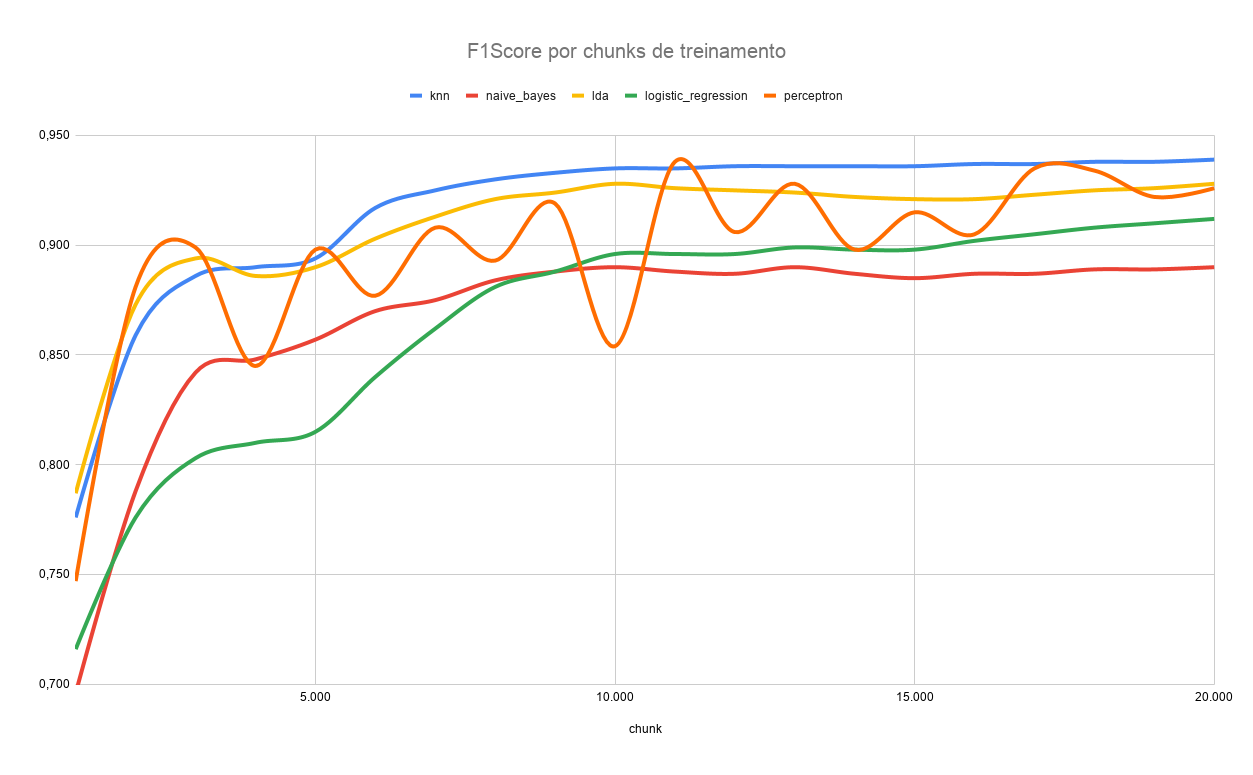
\includegraphics[width=30em]{images/image_comparacao_classificadores.png}
  \caption{Comparação dos Classificadores}
  \label{fig:comparacao_classificadores}
\end{figure}

Destaca-se o comportamento do classificador \textit{perceptron}, que apesar da tendência crescente, mostra uma variação de resultados durante todos os experimentos. Isso acontece por sua por sua característica natual chamada de \textit{Cathastrophic Forgetting}, que acaba ``esquecendo'' os resultados anteriores quando não são frequentemente revisitados nos cálculos. Nota-se ainda, que ao relizar treinamentos com \textit{chunks} maiores, entre $15.000$ e $20.000$, as variações são menores e os resultados são melhores.

Em geral para os classificadores \textit{logistic\_regression}, \textit{naive\_bayes}, \textit{lda} e \textit{knn} a estabilização na melhora dos resultaods aconteceu nos testes com $10.000$ registros usados para o treinamento.

\subsubsection{Classificador que tem o melhor desempenho com poucos dados}

Ainda analisando o gráfico da Figura \ref{fig:comparacao_classificadores}, pode-se notar que o classificador que obteve melhor desempenho com poucos dados foi o \textit{perceptron}, seguido do \textit{lda} e \textit{knn}.

\subsubsection{Classificador que tem melhor desempenho com todos os dados}

O classificador \textit{knn} conseguiu o melhor resultado com todos os dados, conseguindo um F1Score e Acurácia de $0,939$, utilizando os $20.000$ dados de treinamento.

\subsubsection{Classiticador mais rápido}

O classificador mais rápido foi o \textit{perceptron}, que com em apenas $5,5s$ conseguiu obter F1Score e Acurácia de $0,938$.

\subsection{Análise das matrizes de confusão}

Para a análise das matrizes de confusão, foram consideradas as matrizes que tiveram o treinamento com toda a base ($20.000$ registros). Excluindo a diagonal com os acertos, criou-se os gráficos da Figura \ref{fig:comparacao_conf_mat}, no qual a variação de cor das células (em uma escala de azul) é definida por seu valor.

As imagens analisadas são representações manuscritas de dígitos de 10 categorias diferentes, que representam os número decimais $0,1,2,3,4,5,6,7,8,9$. Com isso, observa-se que em várias células os erros são compartilhados entre os classificadores. Isso se deve pois, as confusões são encontradas em números com o formato semelhante, como por exemplo, a confusão entre $(3,5)$ que possui um alto índice de falhas nos classificadores \textit{knn}, \textit{lda} e \textit{logistic\_regression}, mas menos expressivo nos classificadores \textit{naive\_bayes} e \textit{perceptron}.

Como destaques pode-se observar que o \textit{knn} é o que apresenta as falhas de forma distribuída.

Outro destaque é o classificador \textit{perceptron} que possui os erros distruídos de forma esparçada, com muitos erros do mesmo tipo.

\begin{figure}[!htb]
  \centering
  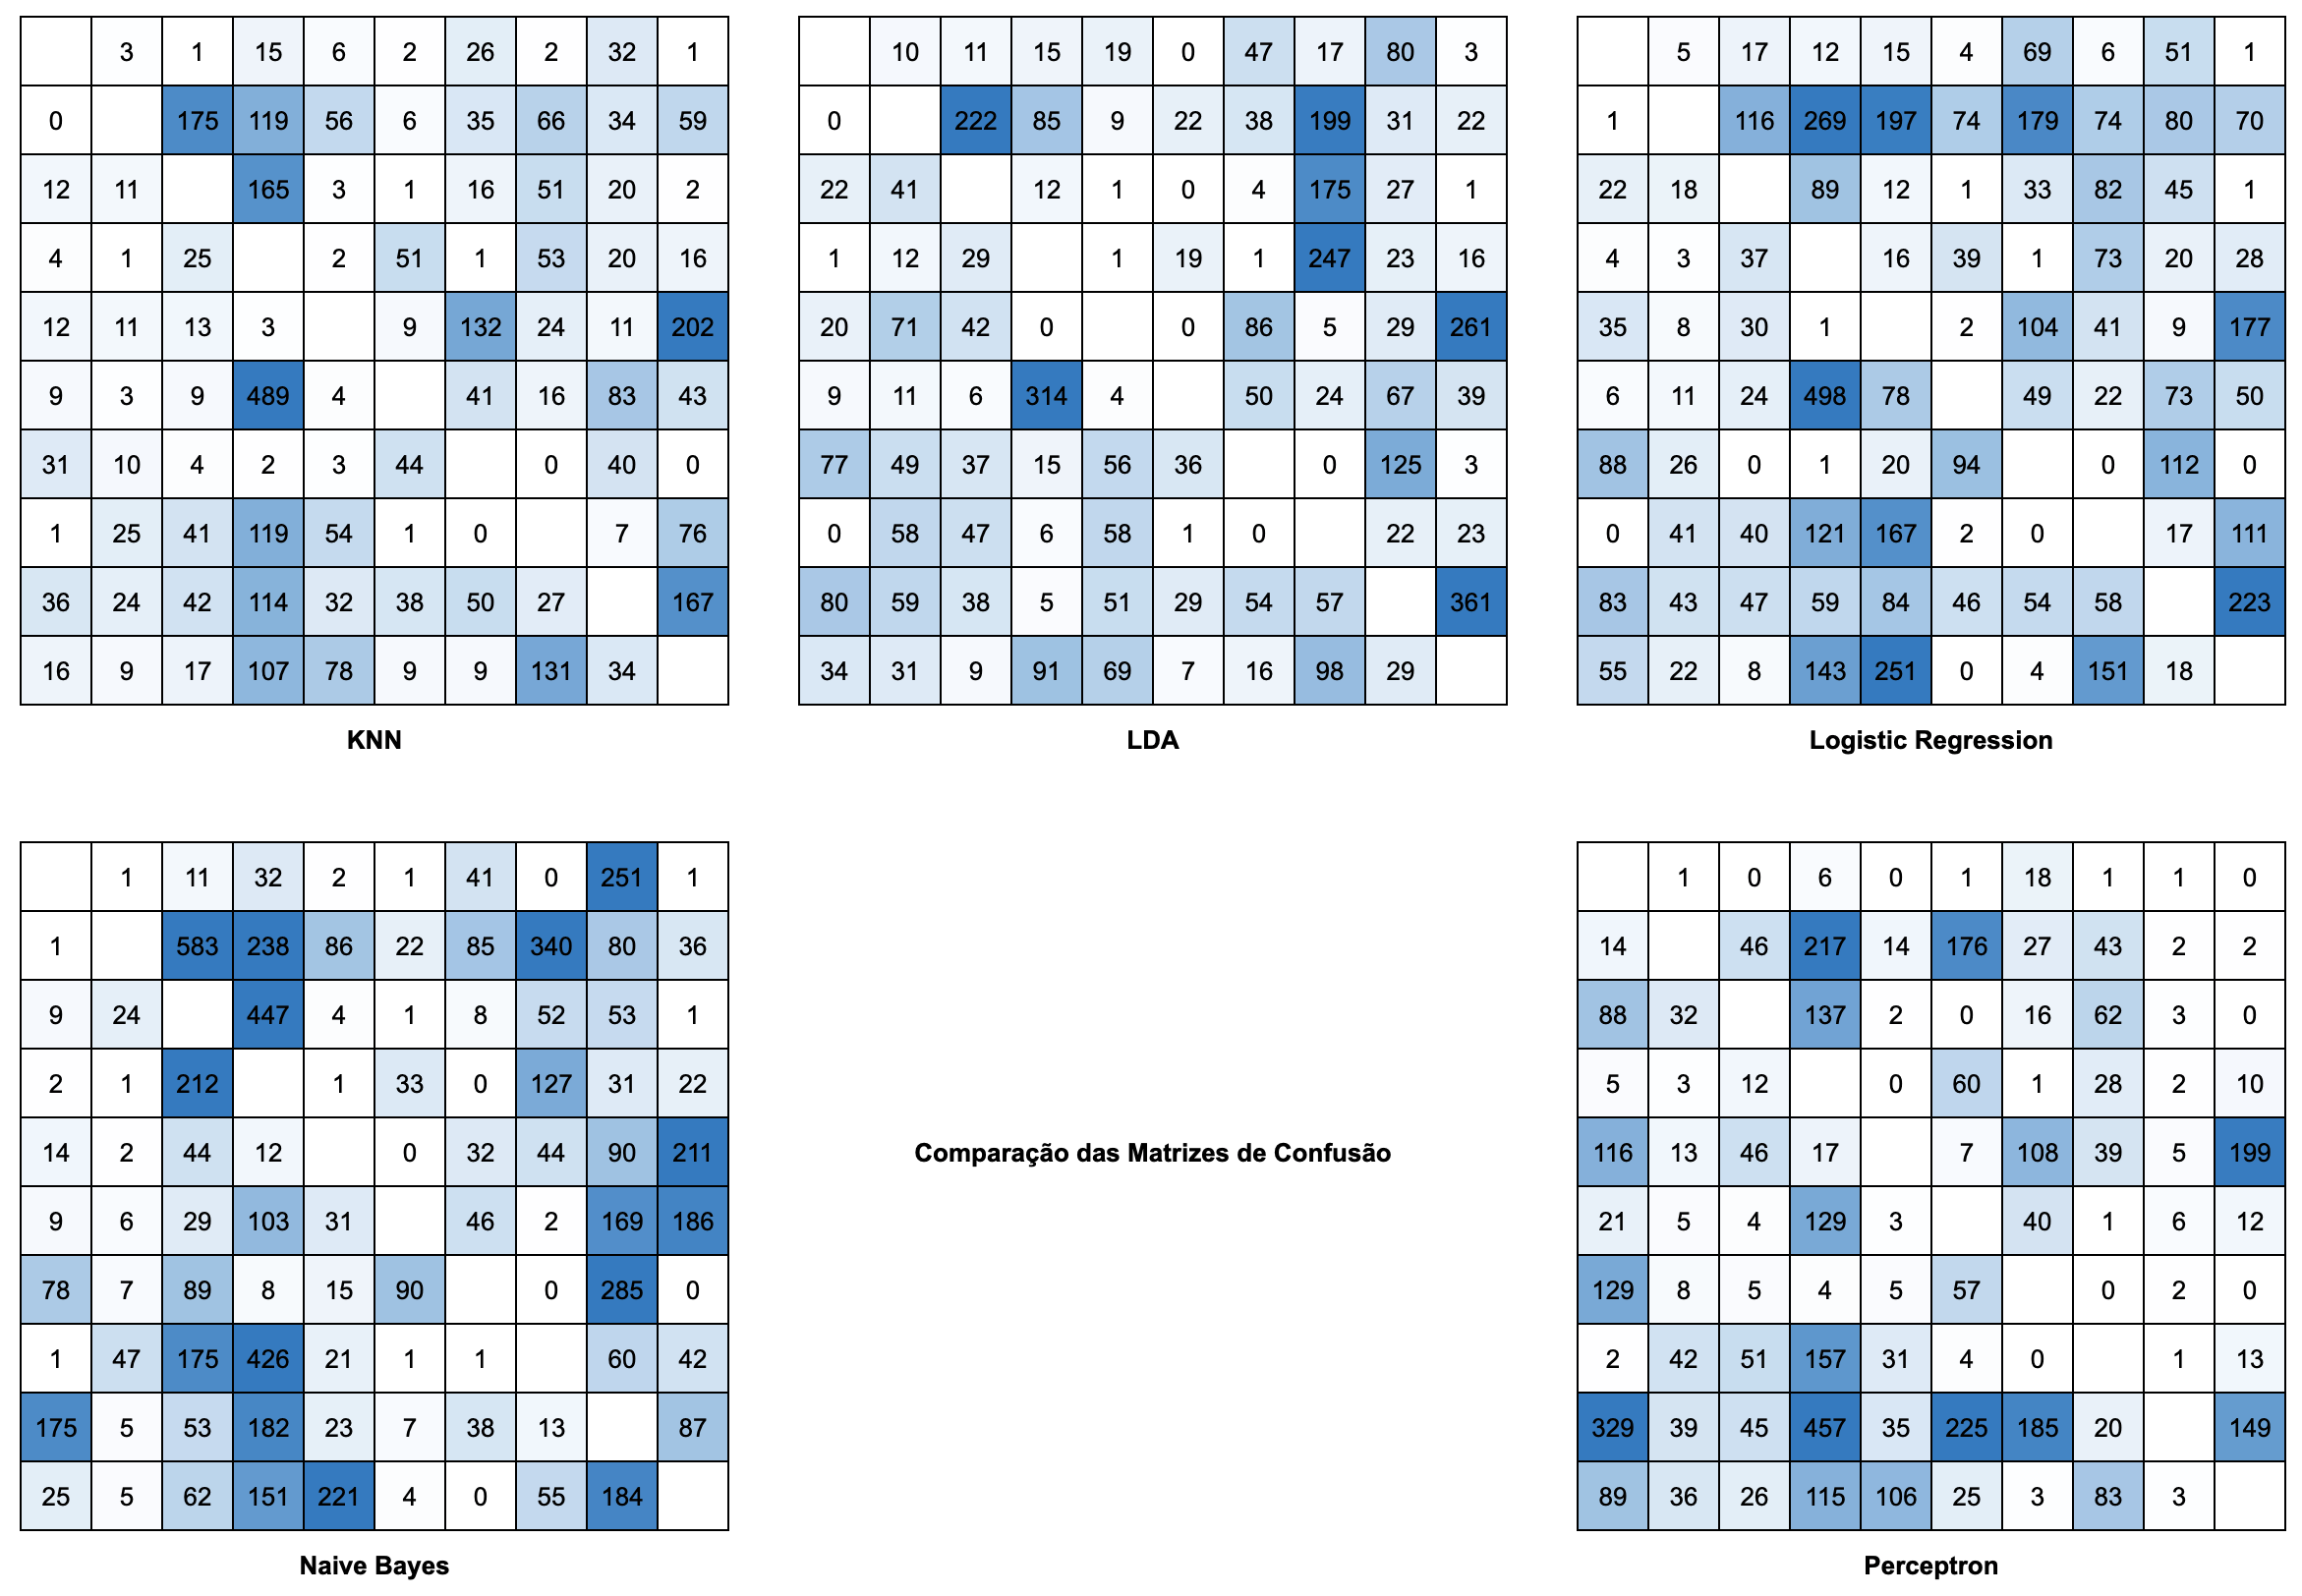
\includegraphics[width=30em]{images/image_comparacao_conf_mat.png}
  \caption{Comparação das Matrizes de Confusão}
  \label{fig:comparacao_conf_mat}
\end{figure}

\subsection{Código Fonte}

Os códigos preparados podem ser analisados através do repositório: https://github.com/diogocezar/machine-learning/tree/master/lab2/src

\end{document}